\subsection{Clarke Transformation and Park Transformation}

% ************************** Clarke Transformation ***********************************
\subsubsection*{Clarke Transform}

Equation \ref{eq:clarke_transformation} implemented in c.

\begin{lstlisting}[style=c, caption=Embedded Clarke Transformation., label=code:clarke]
/* The Clarke function */
void clarke(double *iAlpha, double *iBeta, double iA, double iB, double iC){
	// Power Variant Version
	*iAlpha = TWO_THIRDS * iA - ONE_THIRD * iB - ONE_THIRD * iC;
	*iBeta  = ONE_OVER_SQRT_THREE * iB - ONE_OVER_SQRT_THREE * iC;
}
\end{lstlisting}

% ************************** Park Transformation ***********************************
\subsubsection*{Park Transform}
Equation \ref{eq:park_transformation} implemented in c.

\begin{lstlisting}[style=c, caption=Embedded Park Transformation., label=code:park]
/* The Park function */
void park(double *iD, double *iQ, double iAlpha, double iBeta, double angle){
	const double cosAngle = fastCos(angle);
	const double sinAngle = fastSin(angle);
	*iD = cosAngle * iAlpha + sinAngle * iBeta;
	*iQ = -sinAngle * iAlpha + cosAngle * iBeta;
}
\end{lstlisting}


% ************************** Inverse Park Transformation ***********************************
\subsubsection*{Inverse Park Transform}

Equation \ref{eq:inverse_park_transformation} implemented in c.

\begin{lstlisting}[style=c, caption=Embedded Inverse Park Transformation., label=code:inverse_park]
/* The inverse Park function */
void invPark(double *iAlpha, double *iBeta, double iD, double iQ, double angle){
	const double cosAngle = fastCos(angle);
	const double sinAngle = fastSin(angle);
	*iAlpha = cosAngle * iD - sinAngle * iQ;
	*iBeta  = sinAngle * iD + cosAngle * iQ;
}
\end{lstlisting}



% ************************** Inverse Clarke Transformation ***********************************
\subsubsection*{Inverse Clarke Transform}

Equation \ref{eq:inverse_clarke_transformation} implemented in c.

\begin{lstlisting}[style=c, caption=Embedded Inverse Clarke Transformation., label=code:inverse_clarke]
/* The inverse Clarke function */
void invClarke(double *iA, double *iB, double *iC, double iAlpha, double iBeta){
	// Power Variant Version
	*iA = iAlpha;
	*iB = -HALF * iAlpha + SQRT_THREE_OVER_TWO * iBeta;
	*iC = -HALF * iAlpha - SQRT_THREE_OVER_TWO * iBeta;
}
\end{lstlisting}

\subsubsection{Sine and Cosine}
The trigonometric functions sine and cosine are implemented with a look-up table to improve performance. The sine function looks up a given angle in the table to find the output of the function. The cosine uses the sine function but offset the angle by $90 ^{\circ}$. 

To limit the amount of memory used only one value is saved per degree which results in $360$ saved values of type \textit{double} which is $8$ bytes resulting in $2880 bytes \sim 3kB$ used.
The maximum error that can exist because of the quantization is the biggest step between two values in the data set. 
The largest error is where the sinus has the biggest slope, and this is where it crosses the x-axis. The error is positive when the slope is positive and negative when the slope is negative. The maximum error is $\pm 1.75 \%$ as can be seen on figure \ref{fig:sinus_lookup_error}. 
\begin{figure}[H]
	\centering
	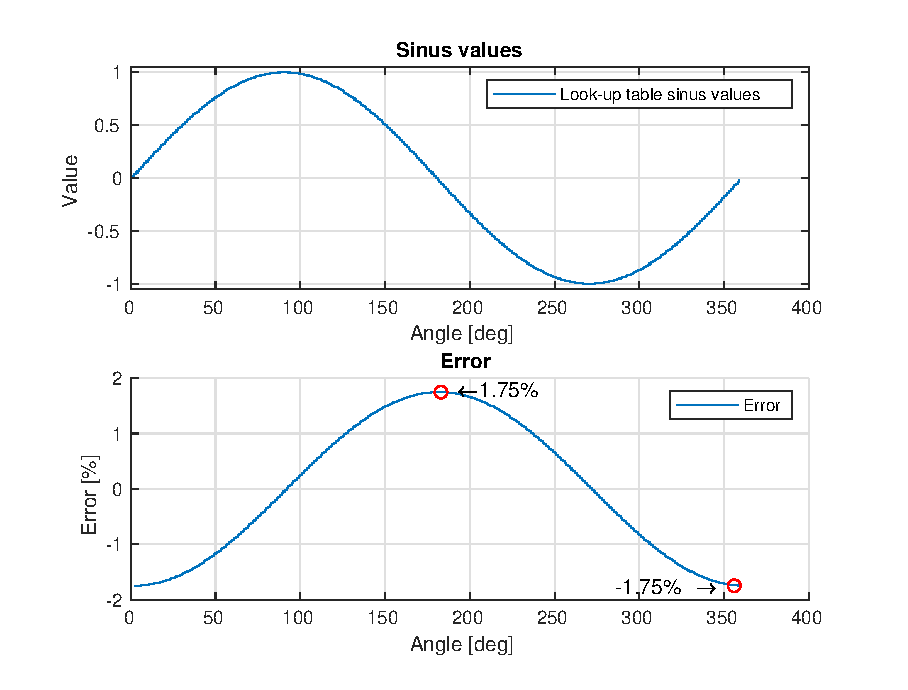
\includegraphics[width=0.6 \textwidth]{pictures/software/sinus_lookup_error.eps}
	\caption{Error between the real sinus value and the look-up table value.}
	\label{fig:sinus_lookup_error}
\end{figure}


\begin{lstlisting}[style=c, caption=Implementation lookup tables., label=code:lookup_table]
/* Sinus lookup table */
#define SIN_N 		360	 // Number of data points in the sinus constant array
const double sinusValues[] = {0,0.0174524064372835,0.0348994967025010,...};

/* Function that returns sin(angle) */
double fastSin(double angle){
	unsigned int index = (unsigned int)angle;       // Truncate decimals
	return (double)sinusValues[index % SIN_N];      // 
}	

/* Function that returns cos(angle) */
double fastCos(double angle){
	double newAngle = (double)((int)(angle + 90) % (int)360);
	return (double)fastSin(newAngle);
}
\end{lstlisting}